\documentclass[11pt]{article}
\usepackage{amsmath,amssymb,amsthm}
\usepackage[margin=1in]{geometry}
\usepackage{graphicx}
\usepackage{booktabs}
\usepackage{longtable}
\usepackage{tikz}
\usetikzlibrary{calc,positioning}
\setlength{\emergencystretch}{2.5em}
\usepackage{hyperref}
\hypersetup{colorlinks=true, linkcolor=black, citecolor=black, urlcolor=blue}

\newtheorem{theorem}{Theorem}
\newtheorem{proposition}[theorem]{Proposition}
\newtheorem{lemma}[theorem]{Lemma}
\newtheorem{corollary}[theorem]{Corollary}
\theoremstyle{definition}
\newtheorem{definition}[theorem]{Definition}
\newtheorem{remark}[theorem]{Remark}

\newcommand{\per}{\operatorname{per}}
\renewcommand{\deg}{\operatorname{deg}}
\newcommand{\bell}{\ell}
\newcommand{\Fs}{F^{\ast}}
\newcommand{\lean}[1]{\texttt{#1}}

\title{The maximum Laplacian ratio of a tree:\\
a complete answer to a question of Brualdi and Goldwasser,\\
kernel-checked in Lean}
\author{Peter W.\ Murphy, MD}
\date{26 September 2026 \quad (preprint, not yet refereed)}

\begin{document}
\maketitle

\begin{abstract}
For a tree $T$ with Laplacian $L(T)$, Brualdi and Goldwasser (1984) introduced the
\emph{Laplacian ratio} $\pi(T)=\per L(T)/\prod_v\deg v$ and asked which tree on $n$ vertices
maximizes it. We answer the question for every $n$. For every $n\ge 4$ the maximum is attained by a
\emph{spider of cherry arms}: a centre carrying pendant paths of length two (cherries) and
\emph{arms}, an arm being a vertex that carries cherries. For $n\ge 492$ the centre carries only arms,
almost all with five cherries, and the exceptional arms are fixed by $6(n-1)\bmod 11$ through an explicit
rule; for $4\le n\le 491$ the maximizer is given by an explicit table. Along the way we determine the
exact exponential growth rate of the maximum,
$\tfrac{64}{621}\rho^{n}\le\max_{|T|=n}\pi(T)\le 2\rho^{n-1}$ with $\rho=(621/64)^{1/11}$, and prove the
sharp inequality behind it: every pendant subtree $b$ has matching weight at most $\rho^{|b|}$, with
equality exactly for the five-cherry arm. The whole argument is formalized in Lean~4 with Mathlib and
checked by the Lean kernel, depending only on Lean's three standard axioms. Large parts of it are
certificates: exact data produced by untrusted generators and checked by the kernel. We describe the
mathematics, the certificates, how the kernel checks them, and how to reproduce every step.
\end{abstract}

\section{Introduction}

Let $T$ be a tree on $n\ge2$ vertices, $D$ its diagonal degree matrix, $A$ its adjacency matrix and
$L(T)=D-A$ its Laplacian. Brualdi and Goldwasser~\cite{BG1984} studied the permanent of $L(T)$ and the
\emph{Laplacian ratio}
\[
  \pi(T)=\frac{\per L(T)}{\prod_{v\in V(T)}\deg v}.
\]
They showed $\pi(T)\ge 2$, with equality exactly for the star, and asked for the \emph{maximum} over
trees on $n$ vertices. Wu, Dong and Lai~\cite{WDL2025} conjectured that the maximizer is a particular
subdivided star. Pant~\cite{Pant2026} refuted that conjecture with explicit families of caterpillars
whose spine vertices each carry many pendant paths of length two, and left the question open.

This paper answers it for every $n$.

\begin{definition}[cherries, arms, spiders]
A \emph{cherry} is a pendant path of length two. For $j\ge1$ an \emph{arm} $A_j$ is a vertex, adjacent
to the centre, that carries $j$ cherries and nothing else; it has $2j+1$ vertices. We write $A_0$ for
a leaf adjacent to the centre. A \emph{spider of cherry arms} (in this paper, simply a \emph{spider})
is a tree with a vertex, the \emph{centre}, all of whose branches are leaves, cherries or arms. We write
$C^{c}A_{j_1}A_{j_2}\cdots$ for the spider whose centre carries $c$ cherries and arms
$A_{j_1},A_{j_2},\dots$
\end{definition}

\begin{figure}[t]\centering
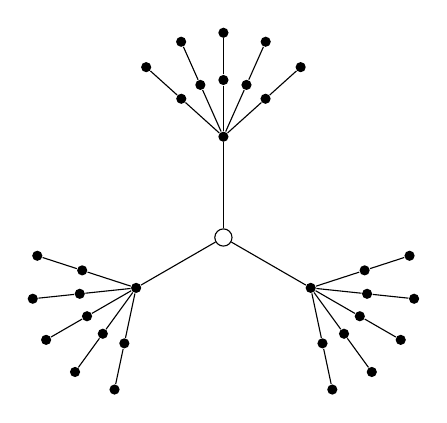
\begin{tikzpicture}[scale=0.8,
  v/.style={circle,fill=black,inner sep=1.3pt},
  c/.style={circle,draw=black,fill=white,inner sep=2.2pt}]
  \node[c] (o) at (0,0) {};
  \foreach \a/\ang in {1/90,2/210,3/330} {
    \node[v] (a\a) at (\ang:1.6) {};
    \draw (o)--(a\a);
    \foreach \k in {0,...,4} {
      \pgfmathsetmacro{\t}{\ang-48+24*\k}
      \node[v] (m\a\k) at ($(a\a)+(\t:0.9)$) {};
      \node[v] (l\a\k) at ($(a\a)+(\t:1.65)$) {};
      \draw (a\a)--(m\a\k)--(l\a\k);
    }
  }
\end{tikzpicture}
\qquad
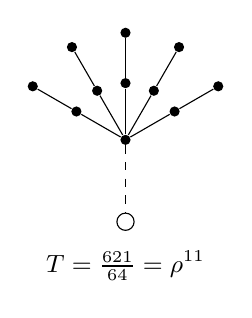
\begin{tikzpicture}[scale=0.8,
  v/.style={circle,fill=black,inner sep=1.3pt},
  c/.style={circle,draw=black,fill=white,inner sep=2.2pt}]
  \node[v] (a) at (0,0) {};
  \node[c] (p) at (0,-1.3) {};
  \draw[dashed] (a)--(p);
  \foreach \k in {0,...,4} {
    \pgfmathsetmacro{\t}{30+30*\k}
    \node[v] (m\k) at (\t:0.9) {};
    \node[v] (l\k) at (\t:1.7) {};
    \draw (a)--(m\k)--(l\k);
  }
  \node at (0,-2.0) {\small $T=\tfrac{621}{64}=\rho^{11}$};
\end{tikzpicture}
\caption{Left: the spider $A_5^{3}$ on $n=34$ vertices (centre drawn open). Right: the five-cherry arm
$A_5$, an 11-vertex pendant subtree whose matching weight is exactly $\rho^{11}$; it is the unique
pendant subtree attaining the sharp bound of Theorem~\ref{thm:sharp}.}
\label{fig:spider}
\end{figure}

\begin{theorem}[main theorem]\label{thm:main}
For every $n\ge4$ the tree $\mathrm{bgMax}(n)$ below has $n$ vertices and maximizes $\pi$ over all trees
on $n$ vertices.
\begin{enumerate}
\item For $n\ge 492$, put $s=6(n-1)\bmod 11$. The centre of $\mathrm{bgMax}(n)$ carries only arms, and
  all of them are $A_5$ except:
  \begin{itemize}
  \item $s\in\{1,2,3,4\}$: $s$ arms are $A_6$; except that for $s=3$ with $n\le722$ and for $s=4$ with
    $n\le 2319$, instead $11-s$ arms are $A_4$;
  \item $s\in\{5,\dots,10\}$: $11-s$ arms are $A_4$.
  \end{itemize}
\item For $4\le n\le 491$, $\mathrm{bgMax}(n)$ is the spider listed in Appendix~\ref{app:table}.
\end{enumerate}
For $n\le3$ there is only one tree on $n$ vertices.
\end{theorem}

The exceptional counts are forced by vertex counting: $|A_4|=9$, $|A_5|=11$, $|A_6|=13$, and
$n-1\equiv 2s\pmod{11}$, so replacing $A_5$'s by $s$ copies of $A_6$, or by $11-s$ copies of $A_4$,
uses up the residue. Figure~\ref{fig:spider} shows the building block.

Theorem~\ref{thm:main} is the Lean theorem
\begin{verbatim}
theorem R3Cert.BGMaximizerAll.bg_maximizer_all (n : Nat) (h4 : 4 <= n) :
    usize (bgMax n) = n /\ forall t : UTree,
      usize t = n -> Aobj t <= Aobj (bgMax n)
\end{verbatim}
together with its companion \lean{bg\_maximizer\_all\_perm}, which states the inequality literally
for $\per(L)/\prod\deg$ of the realized simple graphs (\S\ref{sec:lean}).

\paragraph{Why five cherries.} The number $\rho=(621/64)^{1/11}\approx1.22948$ is the exact exponential
growth rate of the maximum.

\begin{theorem}[growth rate]\label{thm:growth}
For every $n\ge1$,
$\displaystyle \frac{64}{621}\,\rho^{n}\ \le\ \max_{|T|=n}\pi(T)\ \le\ 2\,\rho^{\,n-1}.$
\end{theorem}

The upper bound comes from a sharp inequality for pendant subtrees (Theorem~\ref{thm:sharp}): every
pendant subtree $b$ contributes a factor at most $\rho^{|b|}$, with equality only for the five-cherry
arm. A maximizer therefore uses as many five-cherry arms as the arithmetic of $n$ allows, and the whole
difficulty is in the lower-order terms. Pant's families grow like $(3/2)^{n/2}\approx1.2247^{n}$, just
below $\rho$.

\paragraph{How the proof goes.} The ratio is a weighted matching count, which a cavity recursion
evaluates on rooted trees (\S\ref{sec:cavity}). Rooting a tree at a vertex of maximum degree, we show
that any tree which is not a spider is strictly beaten by some spider of the same size
(\S\ref{sec:reduction}). The spiders form an explicit family with a closed-form value, and we solve the
optimization over it exactly (\S\ref{sec:spiders}). Each step is split by size:

\begin{center}
\small
\begin{tabular}{@{}lp{0.42\textwidth}p{0.33\textwidth}@{}}
\toprule
$n$ & reduction to spiders & best spider \\
\midrule
$4$--$6$ & \multicolumn{2}{p{0.78\textwidth}}{exact rational evaluation of every tree} \\
$7$--$149$ & envelope certificate (degree $\le 23$) + high-degree theorem & table sweep \\
$150$--$491$ & credited rate cells + high-degree theorem & table sweep \\
$\ge 492$ & rate cells + high-degree theorem & exchange lemmas + 223 polynomial certificates \\
\bottomrule
\end{tabular}
\end{center}

\paragraph{Status.} Every step is formalized in Lean~4 with Mathlib~\cite{Mathlib} and checked by the Lean kernel; the headline
theorems depend only on \lean{propext}, \lean{Classical.choice} and \lean{Quot.sound}, with no
\lean{sorry}, no \lean{native\_decide} and no added axioms. The result has not yet been refereed. The
kernel certifies the deductions; what a reader must still check is that the formal statement says what
we claim it says, and \S\ref{sec:lean} is written to make that check easy. The development was carried
out with extensive help from an AI system (see the acknowledgements); for that reason we have tried to
make every claim checkable by machine and every certificate reproducible from scratch.

\section{The ratio as a matching sum, and the cavity recursion}\label{sec:cavity}

\begin{theorem}[\cite{BG1984,Pant2026}]\label{thm:matchsum}
For a tree $T$,
\[
  \per L(T)=\sum_{M}\ \prod_{v\notin V(M)}\deg v,
  \qquad\text{hence}\qquad
  \pi(T)=\sum_{M}\ \prod_{uv\in M}\frac{1}{\deg u\,\deg v},
\]
the sums running over all matchings $M$ of $T$, including the empty one.
\end{theorem}
\begin{proof}
A term $\prod_i L_{i,\sigma(i)}$ of the permanent is nonzero only if every $i$ is fixed by $\sigma$ or
sent to a neighbour. The non-trivial cycles of $\sigma$ then run along edges of $T$; since $T$ has no
cycles, they are transpositions along edges, that is, a matching $M$. A fixed point contributes
$L_{ii}=\deg i$ and a matched edge contributes $L_{ij}L_{ji}=1$.
\end{proof}

In Lean this is \lean{pi\_eq\_msum} (file \lean{Matching.lean}), proved for any finite acyclic simple
graph; the bridge \lean{pi\_utree} specializes it to the trees of the formalization.

The weighted matching sum is a monomer-dimer partition function in the sense of
Heilmann and Lieb~\cite{HL1972}, with edge weights $1/(\deg u\deg v)$.

\paragraph{Planted branches.} A \emph{planted branch} $b$ is a rooted tree whose root will be attached to
one further vertex, its parent. All degrees are measured in the final tree, so the root of $b$ has degree
$d_b=(\text{number of children})+1$. Let $T_b$ be the matching sum of Theorem~\ref{thm:matchsum}
restricted to $b$, and $T^{\circ}_b$ the same sum over matchings that leave the root of $b$ unmatched. Put
$y_b=T^{\circ}_b/(d_bT_b)$. Splitting on whether, and to which child, the root is matched gives
\begin{equation}\label{eq:cavity}
  T_b=\Big(\prod_{c}T_c\Big)\frac{d_b+R_b}{d_b},\qquad
  y_b=\frac{1}{d_b+R_b},\qquad R_b=\sum_c y_c,
\end{equation}
the products and sums running over the children $c$ of the root. A leaf has $T=1$, $y=1$. For a tree
rooted at a vertex with $k$ children,
\begin{equation}\label{eq:root}
  \pi(T)=\Big(\prod_{c}T_c\Big)\Big(1+\frac{R}{k}\Big),\qquad R=\sum_c y_c .
\end{equation}
Since \eqref{eq:cavity} multiplies one factor per vertex, $\log T_b=\sum_{v\in b}\log(1+R_v/d_v)$.

\paragraph{Atoms.} Iterating \eqref{eq:cavity}: a cherry has $T=\tfrac32$ and $y=\tfrac13$. The arm $A_j$
has $d=j+1$ and $R=j/3$, so
\begin{equation}\label{eq:arm}
  T(A_j)=\Big(\frac32\Big)^{j}\frac{4j+3}{3(j+1)},\qquad y(A_j)=\frac{3}{4j+3}.
\end{equation}
In particular $T(A_5)=(3/2)^5\cdot\tfrac{23}{18}=\tfrac{621}{64}$. The per-vertex rates are
\[
\begin{array}{c|ccccccc|c}
 & A_1 & A_2 & A_3 & A_4 & A_5 & A_6 & A_7 & \text{cherry}\\\hline
\frac{\log T}{\#\text{vertices}} & 0.18654 & 0.20232 & 0.20565 & 0.2064721 & \mathbf{0.2065862} & 0.2064696 & 0.20628 & 0.2027326
\end{array}
\]
and $\log T(A_j)/(2j+1)\to\tfrac12\log\tfrac32$, the cherry value, as $j\to\infty$. The five-cherry arm
is the unique best, with $A_4$ and $A_6$ just behind.

\section{The sharp ceiling and the growth rate}\label{sec:ceiling}

Write $\Fs=\tfrac1{11}\log\tfrac{621}{64}=\log\rho$ and, for a planted branch $b$ with $|b|$ vertices,
$\bell(b)=\log T_b-|b|\Fs$.

\begin{theorem}[sharp ceiling]\label{thm:sharp}
Every planted branch $b$ satisfies $T_b\le\rho^{|b|}$, that is $\bell(b)\le0$, with equality if and only
if $b$ is the five-cherry arm $A_5$.
\end{theorem}

In Lean: \lean{R3Cert.BGSCL.bg\_sharp}.

\begin{proof}[Outline]
\emph{Telescoping.} By the remark after \eqref{eq:root}, $\bell(b)=\sum_{v\in b}e_v$ with
$e_v=\log(1+R_v/d_v)-\Fs$. Suppose $\varrho\ge0$ is a function of a vertex's local state with
\begin{equation}\label{eq:sub}
  e_v+\varrho(v)\ \le\ \sum_{c\text{ child of }v}\varrho(c)\qquad\text{for every vertex }v.
\end{equation}
Summing \eqref{eq:sub} over $b$ telescopes to $\bell(b)\le-\varrho(\mathrm{root})\le0$. In the language
of ergodic optimization $\varrho$ is a \emph{subaction}.

\emph{The witness.} We use an explicit subaction $\varrho_{\mathrm{wit}}$ depending on a vertex's
number of children and on its message $y$: it equals $\Fs$ at a leaf, is affine in $y$ at vertices with one,
two or three children, and vanishes at vertices with four or more. Three constraints are tight, and they are exactly the three vertex types of
$A_5$: leaf, cherry vertex, and the arm vertex with five cherries. (That the extremal structure is a
finite periodic pattern is what makes a finite piecewise-affine subaction possible; compare
\cite{Bousch2001}.) Their consistency is the identity
$(3/2)^5\cdot\tfrac{23}{18}=\tfrac{621}{64}$, that is $27\cdot23=621$. Every other instance of
\eqref{eq:sub} holds with rational slack. The verification splits into finitely many cells by degree
(among them 35 cells for vertices with four children, and a tail wrapper for high degree), each an inequality
between rational envelopes and a rational enclosure of a logarithm (Taylor or $\operatorname{atanh}$
series with explicit remainder); see \lean{BGSCLSubaction*.lean}.

\emph{Equality.} If $\bell(b)=0$ then every cell along $b$ is tight. The root cell is tight only at
degree six, and at degree six only when all five children are cherries: one non-cherry child makes the
cell strict, using the strict inequality $2\Fs-\log\tfrac32<\tfrac1{96}$. That inequality is where
strictness enters; at degree three the non-strict version is exactly tight.
\end{proof}

\begin{proof}[Proof of Theorem~\ref{thm:growth}]
Root $T$ anywhere. In \eqref{eq:root} each child $c$ is a planted branch, so $\prod_cT_c\le\rho^{n-1}$
by Theorem~\ref{thm:sharp}; and each $y_c\le1$, so $1+R/k\le2$. For the lower bound, take a centre
carrying $K=\lfloor (n-1)/11\rfloor$ arms $A_5$, and fill the remaining at most ten vertices with
cherries and at most one leaf; each $T\ge1$, so $\pi\ge\rho^{11K}\ge\tfrac{64}{621}\rho^{n}$.
In Lean: \lean{R3Cert.Step3.bg\_max\_growth}.
\end{proof}

\section{Every maximizer is a spider}\label{sec:reduction}

Root a tree at a vertex of maximum degree $k$; call its children $b_1,\dots,b_k$. Every vertex then has at
most $k-1$ children. Rerooting preserves $\pi$ and the vertex count (\lean{RerootRel},
\lean{exists\_maxRooted}). The \emph{atoms} are the leaf, the cherry and the arms $A_j$; the tree is a
spider centred at the root exactly when every $b_i$ is an atom. Taking logarithms in \eqref{eq:root},
\begin{equation}\label{eq:lagrange}
  \log\pi-(n-1)\Fs=\sum_{i=1}^{k}\bell(b_i)+\log\Big(1+\frac{S}{k}\Big),\qquad S=\sum_i y_{b_i}.
\end{equation}
By Theorem~\ref{thm:sharp} every term of the sum is $\le0$. The task is to show that a non-atom child costs
more than any possible gain in the last term, measured against the best spider of the same size. We
compare with explicit spiders: the $A_5/A_4$ spider (with $q\equiv5(n-1)\pmod{11}$ arms $A_4$ and the rest
$A_5$) satisfies
\begin{equation}\label{eq:floor}
  \log\pi-(n-1)\Fs\ \ge\ \log\tfrac{26}{23}-\tfrac{10}{960},
\end{equation}
because $A_4$ has $y=\tfrac3{19}>\tfrac3{23}=y(A_5)$ and each $A_4$ costs little.

\paragraph{High degree ($k\ge24$).} Use the tangent of $\log(1+S/k)$ at $S/k=3/23$, which prices each
unit of message at $\mu=\tfrac{23}{26k}\le\tfrac{23}{624}$. For $V_\mu(b)=\bell(b)+\mu y_b$ we show that on
this range of $\mu$ the arm $A_5$ is the envelope of $V_\mu$ over all branches, and every non-atom lies
below it by at least $\tfrac1{75}$ (the observed minimum is $0.01452$, at a vertex carrying five
cherries and an $A_4$). This reduces, through the subaction, to three per-vertex statements, each proved
with rational tangent certificates and degree-six Taylor enclosures of $\log$. Hence a max-degree rooting
with a non-atom child has $\log\pi-(n-1)\Fs\le\log\tfrac{26}{23}-\tfrac1{75}$, below
\eqref{eq:floor}. This settles $k\ge24$ for $n\ge91$ (\lean{spider\_dominates\_highDegree\_uncond}); for
$25\le n\le90$ we compare with the table spider instead, by a kernel-checked inequality at each $n$
(\lean{BGHighDegreeSmall.highDegree\_small}).

\paragraph{Low degree, large $n$ ($k\le23$, $n\ge492$).} Here we trade the subaction's slack for a
\emph{linear deficit}. A \emph{rate cell} with degree cap $D$ and rate $\alpha$ is a per-vertex inequality
which, telescoped as in \eqref{eq:sub}, yields
\[
  \bell(b)+\varrho_{\mathrm{wit}}(b)\ \le\ -\alpha|b|\qquad\text{for every non-atom branch }b
  \text{ with at most }D-1\text{ children per vertex.}
\]
We use $D=23$ with $\alpha=\tfrac1{3700}$ (root degree $6$ to $23$), and $D=5,4,3,2$ with
$\alpha=\tfrac1{2100},\tfrac1{660},\tfrac1{420},\tfrac1{135}$ (root degree $5,4,3,2$). There are 32 rate
cells and 22 root cells; the tightest margin is $2.8\cdot10^{-4}$. Then
$\log\pi-(n-1)\Fs\le R_k-\alpha(n-1)$ with $R_k\in[0.208,0.319]$, which falls below \eqref{eq:floor} once
$n-1\ge491$ (\lean{spider\_dominates\_lowDegree\_uncond}).

\paragraph{Low degree, $150\le n\le491$.} The same scheme with two refinements: in a tree of maximum
degree $\le D$ every message satisfies $y\ge 1/(2D-1)$, which narrows the per-cell ranges; and non-atom
branches carry a \emph{credit} $\kappa$ depending on their number of children,
$\bell(b)+\varrho_{\mathrm{wit}}(b)\le-\alpha|b|-\kappa(b)$, which they pass to the root. The root is then
bounded by an explicit knapsack over atoms, certified separately for each pair $(k,n)$
(\lean{BGSpiderMidCells*}, \lean{BGSpiderMidRoot*}; \lean{spider\_dominates\_of\_maxDegreeRoot\_150}).

\paragraph{Low degree, $7\le n\le149$: the envelope certificate.} For small $n$ the linear deficit is too
weak, and we instead compute a Bellman envelope. Fix a rational rate $f$ close to $\Fs$ (it cancels between
a tree and a spider of the same size) and a grid of prices $\mu_g$. With
$V_{\mu}(b)=\log T_b-|b|f+\mu y_b$, the tangent of $x\mapsto\log x+\mu/x$ bounds $V_\mu$ at a vertex by a
constant plus $\sum_cV_{\nu}(c)$ at a new price $\nu$ (\lean{BGEnvCert.Tangent}), and a max-plus knapsack
over child sizes bounds the sum. A table $w(m,g)$, indexed by size $m$ and grid point $g$, is a valid
envelope if it satisfies finitely many such inequalities; the envelope theorem
(\lean{BGEnvCert.Envelope}) then gives $V_{\mu_g}(b)\le w(|b|,g)$ for every branch of size $m$ with at
most $C$ children per vertex, and a sharper table for non-atoms. The root inequality with at least one
non-atom child is checked against certified lower bounds for explicit spiders (\lean{BGEnvCert.Spider}).

All tables are stored in fixed point ($34$ fractional bits) and packed into lanes of large natural
numbers, and the checks are Boolean functions that the kernel evaluates. We cover root degrees
$2\le k\le23$ with caps $C\in\{1,\dots,8,12,16,22\}$; roots of degree $\ge24$ are handled by the
high-degree theorems. The certificate is sharded into 57 Lean files (\S\ref{sec:telperion}) and
assembled by \lean{BGEnvCert.AssembleK} into \lean{G149.envcertK}; the result is
\lean{maximizer\_is\_spider\_small}.

\paragraph{$4\le n\le6$.} Every tree is enumerated by a fuel-bounded structural recursion and its value
computed exactly over $\mathbb{Q}$ (\lean{BGMaximizerTiny}).

\begin{theorem}\label{thm:reduction}
For every $n\ge7$, every tree on $n$ vertices that maximizes $\pi$ is, after rerooting at a vertex of
maximum degree, a spider. For $n\ge492$ every tree on $n$ vertices is weakly beaten by a spider on $n$
vertices.
\end{theorem}

In Lean: \lean{maximizer\_is\_spider\_small} ($7\le n\le149$), \lean{BGMax.maximizer\_is\_spider\_150}
($n\ge150$), \lean{BGMax.bg\_spider\_reduction} ($n\ge492$).

\section{The best spider}\label{sec:spiders}

A spider is described up to isomorphism by the multiset of its centre's children. By
\eqref{eq:root} and \eqref{eq:arm} its value has the closed form
\[
  F=\Big(\frac32\Big)^{c+\sum j}\prod_{\text{arms}}\alpha_j\cdot\Big(1+\frac{c/3+\sum b_j}{D}\Big),
  \qquad \alpha_j=\frac{4j+3}{3(j+1)},\quad b_j=\frac{3}{4j+3},
\]
where $c$ is the number of cherries, the product and sum run over the arms (leaves being $A_0$, with
$\alpha_0=b_0=1$), and $D$ is the degree of the centre. In Lean, $F$ is a function on lists of children
over $\mathbb{Q}$, and \lean{Aobj\_spiderU} identifies it with $\pi$ of the realized tree.

\begin{lemma}[balance]\label{lem:balance}
Put $Q_c(x,y)=\alpha_x\alpha_y(c+b_x+b_y)$. For integers $k,t\ge0$,
\[
  Q_c(k+t+1,k+1)-Q_c(k+t+2,k)=\frac{(t+1)\big((c-3)(8k+4t+15)+3\big)}{9(k+1)(k+2)(k+t+2)(k+t+3)}.
\]
Consequently, if $D\ge3$, moving a cherry from an arm to an arm at least two smaller strictly increases
$F$, and in every maximizer with $D\ge3$ all arm sizes (leaves included) differ by at most one.
\end{lemma}

\begin{proof}
The move keeps $n$, $D$ and the power of $\tfrac32$, and multiplies $F$ by
$Q_c(\text{new})/Q_c(\text{old})$ with $c=D+R_0\ge3$, where $R_0$ is the message sum of the other
children. The identity is a polynomial identity (\lean{balance\_identity}).
\end{proof}

Two further exact exchanges are used: two leaves are never better than one cherry
(\lean{F\_leafpair\_lt}), and a general local-exchange criterion that is affine in $R_0$ and so reduces to
two quadratics in $D_0$ (\lean{F\_exchange\_lt}).

\paragraph{$4\le n\le491$.} By Lemma~\ref{lem:balance}, a maximizer with $D\ge3$ is a permutation of a
canonical configuration $(c,s,a,b)$: $c$ cherries, $a$ arms $A_s$ and $b$ arms $A_{s+1}$. Its value has
an exact integer numerator and denominator. For each $n$ the kernel compares every canonical
configuration on $n$ vertices, and every configuration with $D\le2$, against the table entry, by
cross-multiplied inequalities of natural numbers (\lean{BGSpiderTable.spider\_opt\_table}). The sweep is
split into 89 chunk files of about five sizes each. At $n=21$ two non-isomorphic spiders tie
($C^{10}$ and $C^3A_3^2$); the table records $C^3A_3^2$.

\paragraph{$n\ge492$: structure.} Let $l$ be a maximizer of $F$ with $n\ge492$. Then (Lean: \lean{structProp\_492}) the centre has at least three children; there is no arm $A_j$
with $j\ge13$ (split it into $A_{j-11}$ and two $A_5$); none with $7\le j\le12$ (exchange eleven $A_j$ for
$2j+1$ copies of $A_5$, and a global comparison with the rule spider); at most eight cherries (nine
cherries lose to two $A_4$); no arm with $j\le3$; so every arm is $A_4$, $A_5$ or $A_6$, $A_4$ and $A_6$
do not occur together, and there are at most ten of each. The global comparison uses
$(\prod T)^2=(3/2)^{n-1}\prod h$ with $h(\text{cherry})=1$ and $h(A_j)=\tfrac23\alpha_j^2$; its tightest
instance is $24.45<28.43$.

\paragraph{$n\ge492$: the candidates.} A candidate is determined by its counts $(c,k_4,k_5,k_6)$, and
$F=\Phi(c,k_4,k_5,k_6)$ with
$\Phi=(\tfrac32)^{c}G_4^{k_4}G_5^{k_5}G_6^{k_6}\bigl(1+\frac{c/3+k_4B_4+k_5B_5+k_6B_6}{c+k_4+k_5+k_6}\bigr)$,
$G_4=\tfrac{513}{80}$, $G_5=\tfrac{621}{64}$, $G_6=\tfrac{6561}{448}$, $B_4=\tfrac3{19}$, $B_5=\tfrac3{23}$,
$B_6=\tfrac19$. The triple $(c,k_4,k_6)$ fixes the residue class $s$ and hence the rule winner's counts;
after dividing out a common power of $G_5$, the comparison $\Phi(\text{candidate})\le\Phi(\text{winner})$
becomes $P(m)\ge0$ for an explicit quadratic $P$ in the common number $m$ of five-cherry arms. There are
189 triples and 223 certificates: 221 write $P(L+t)$ with nonnegative coefficients in $t$, and two (the
competitions that decide the thresholds $722$ and $2319$) write it in the Bernstein basis on a bounded
interval. Lean checks each identity with \lean{ring} and each sign with \lean{norm\_num}
(\lean{BGSpiderCand.candProp\_492}).

Together these prove Theorem~\ref{thm:main}: Theorem~\ref{thm:reduction} reduces to spiders, and this
section finds the best spider.

\section{The formal statement}\label{sec:lean}

This section is for a reader who wants to check that the Lean theorem means what Theorem~\ref{thm:main}
says. The relevant definitions are short.

\begin{itemize}
\item \lean{UTree} is the type of finite rooted trees, built by \lean{node} from a list of subtrees, and
  \lean{usize} counts vertices. Every finite tree arises, rooted anywhere.
\item \lean{Step3.realize (dtRealize t)} turns $t$ into an explicit edge list, and \lean{aGraph} into a
  Mathlib \lean{SimpleGraph} on its vertex type.
\item \lean{lapl G} is the matrix with $\deg i$ on the diagonal, $-1$ on edges and $0$ elsewhere, and
  \lean{Matrix.permanent} is Mathlib's permanent.
\item \lean{Aobj t} is defined as the matching sum of the realized tree; \lean{pi\_utree} proves
  \[
  \texttt{(lapl (aGraph ...)).permanent / (prod over v of degree v) = Aobj t}.
  \]
\item \lean{bgMax n} is \lean{spiderU (tab n)} for $n\le491$ and \lean{spiderU (W n)} otherwise, where
  \lean{tab} reads the table \lean{BGSpiderTableData.tabData} and \lean{W} implements the rule of
  Theorem~\ref{thm:main}.
\end{itemize}

So \lean{bg\_maximizer\_all\_perm} states, for every $n\ge4$ and every tree $t$ on $n$ vertices, that
$\per L/\prod\deg$ of $t$ is at most that of $\mathrm{bgMax}(n)$, with the permanent and the degrees read
off the actual graph. The file \lean{AxiomGuard.lean} prints the axioms of the 17 headline theorems.

\paragraph{What is not claimed in Lean.} The Lean theorem gives \emph{a} maximizer. That it is unique up
to isomorphism (except at $n=21$) is established by exact computation for $n\le491$ (below) and for
$n\ge2320$ by an exact rational certificate, but uniqueness is not formalized.

\section{Certificates and Telperion}\label{sec:telperion}

Most of the proof's bulk is data: envelope tables, rate-cell constants, table rows, polynomial
coefficients. We produce it with generators written in Python using exact integer and rational
arithmetic, and we never trust the generators: each certificate is a Lean file whose checks the kernel
evaluates, so a wrong certificate is simply a failed build.

The certificates are packaged with Telperion, a pipeline built on exactly that division of labour: an
untrusted \emph{emitter} produces a certificate, a small adapter renders it as Lean, and the Lean kernel is
the only trusted component. For each certificate family the repository contains the generator, a
\emph{frozen} copy of its output with hashes, and a driver that regenerates the family from scratch and
compares byte for byte, both with the frozen copy and with the files in the formalization:

\begin{center}
\begin{tabular}{@{}lrl@{}}
\toprule
family & Lean files & content \\
\midrule
\texttt{spider\_table} & 91 & table rows and the per-$n$ sweep, $n\le491$ \\
\texttt{envcert\_g149} & 57 & envelope tables, tangents, spider bounds, $7\le n\le149$ \\
\texttt{mid\_cells} & 45 & credited rate cells and root knapsacks, $150\le n\le491$ \\
\texttt{cand\_certs} & 10 & the 223 polynomial certificates, $n\ge492$ \\
\bottomrule
\end{tabular}
\end{center}

\paragraph{Making the kernel do it.} Three facts about the Lean kernel shaped the certificates.
(i) It does not reduce definitions by well-founded recursion efficiently, so every recursive check is
structural, with explicit fuel. (ii) It does not share the evaluation of repeated argument subterms, so a
loop state reused twice is evaluated twice; we emit literal constants and force evaluation of natural
numbers before passing them on (\lean{BGEnvCert.Force}). (iii) Arithmetic in $\mathbb{Q}$ is slow, so large
checks use natural numbers and fixed point, and only small ones use $\mathbb{Q}$. We use
\lean{decide +kernel} and never \lean{native\_decide}, so the compiler is not trusted. Because the kernel
keeps every intermediate term of a declaration in memory, large checks are split into many small
theorems and many files; the heaviest files still need 15--35\,GiB each.

\section{Independent computations}

None of the following is needed for the Lean proof; they are independent checks.

\begin{itemize}
\item \emph{Certified search, $n\le491$.} A bottom-up search over all rooted trees, with no degree cap,
  storing every quantity as an outward-rounded interval and discarding a partial state only when it is
  provably strictly beaten in every completion. Surviving candidates are re-evaluated in exact rational
  arithmetic. For every $n\le491$ the exact maximum equals the table value, and \emph{every} maximizing
  tree is a spider. (952\,s on one core; \texttt{certificates/checks}.)
\item \emph{Brute force.} Exact enumeration of all non-isomorphic trees agrees for $n\le18$.
\item \emph{Spider optimization.} An exhaustive exact optimization over the spider family for
  $n\le2400$, together with an exact rational certificate for $n\ge2320$, agrees with the table and the
  rule; an exact Pareto dynamic programme over the family with no balance assumption agrees for
  $n\le600$.
\end{itemize}

\section{Reproducing the results}

The repository \url{https://github.com/DrMurphyIsIn/brualdi-goldwasser} contains the Lean project
(Lean \texttt{v4.32.0}, Mathlib), the certificate generators with their frozen outputs, and the
Telperion engine.
\begin{verbatim}
cd formalization && lake exe cache get && lake build -j 4
lake env lean AxiomGuard.lean
certificates/verify.sh         # regenerate all certificates, compare
certificates/verify.sh --full  # also the certified search, n <= 491
\end{verbatim}
The full build takes several CPU-hours and needs a machine with at least 64\,GiB of memory.

\section{Limitations}

\begin{itemize}
\item The result has not been refereed. The Lean kernel checks the deductions; the correspondence
  between the formal definitions and the mathematical statement (\S\ref{sec:lean}) is what a human
  reviewer should check.
\item The proof is long and mostly computational. We do not have a short conceptual proof that the
  maximizer is a spider, only per-vertex inequalities verified by certificate, and the thresholds
  ($n=150$, $491$, $492$) are artefacts of the method.
\item Uniqueness is not formalized.
\item The trusted base is the Lean kernel, Mathlib's definitions of the permanent and of simple graphs,
  and our definitions listed in \S\ref{sec:lean}.
\end{itemize}

\section*{Acknowledgements}
The formalization, the certificate generators and much of the exploration were developed with extensive
assistance from Claude, an AI system made by Anthropic, working under the author's direction. The author
takes responsibility for the content. The correctness of the formal proof rests on the Lean kernel, not
on either.

\section*{Licensing}
Mathematics and Lean code: Apache-2.0. This paper: CC-BY-4.0. The vendored Telperion engine: Business
Source License~1.1, free for research, teaching and peer review.

\begin{thebibliography}{9}
\bibitem{BG1984} R.~A.~Brualdi and J.~L.~Goldwasser,
\emph{Permanent of the Laplacian matrix of trees and bipartite graphs},
Discrete Math.\ \textbf{48} (1984), 1--21.
\bibitem{WDL2025} T.~Wu, X.~Dong and H.-J.~Lai,
\emph{Two problems on Laplacian ratios of trees},
Discrete Appl.\ Math.\ \textbf{372} (2025), 224--236.
\bibitem{Pant2026} P.~Pant,
\emph{Counterexamples to a conjecture on Laplacian ratios of trees},
arXiv:2605.14176 (2026).
\bibitem{HL1972} O.~J.~Heilmann and E.~H.~Lieb,
\emph{Theory of monomer-dimer systems},
Comm.\ Math.\ Phys.\ \textbf{25} (1972), 190--232.
\bibitem{Bousch2001} T.~Bousch,
\emph{La condition de Walters},
Ann.\ Sci.\ \'Ec.\ Norm.\ Sup\'er.\ \textbf{34} (2001), 287--311.
\bibitem{Mathlib} The mathlib Community,
\emph{The Lean mathematical library},
CPP 2020, 367--381.
\end{thebibliography}

\appendix
\section{The maximizers for $4\le n\le491$}\label{app:table}

Notation: $C^{c}$ is $c$ cherries at the centre, $A_j^{m}$ is $m$ arms with $j$ cherries, $L$ a leaf at
the centre. The third column is $\pi/\rho^{\,n-1}$, which by Theorem~\ref{thm:growth} lies in
$[\tfrac{64}{621}\rho,\,2]$. At $n=21$, $C^{10}$ ties with the listed tree.
Generated from \texttt{BGSpiderTableData.lean} by \texttt{paper/gen\_table.py}.

{\small
\setlength{\tabcolsep}{4pt}
\begin{longtable}{@{}rlr@{\quad}rlr@{\quad}rlr@{}}
\toprule
$n$ & maximizer & $\pi/\rho^{n-1}$ & $n$ & maximizer & $\pi/\rho^{n-1}$ & $n$ & maximizer & $\pi/\rho^{n-1}$\\
\midrule
\endhead
4 & $A_{1}$ & 1.3452 & 167 & $C^{3}$\,$A_{5}^{8}$\,$A_{4}^{8}$ & 1.1378 & 330 & $A_{5}^{25}$\,$A_{4}^{6}$ & 1.1288 \\
5 & $C^{2}$ & 1.3129 & 168 & $C^{3}$\,$A_{5}^{13}$\,$A_{4}^{2}$ & 1.1383 & 331 & $A_{5}^{30}$ & 1.1304 \\
6 & $C$\,$A_{1}$ & 1.2904 & 169 & $C^{3}$\,$A_{5}^{9}$\,$A_{4}^{7}$ & 1.1376 & 332 & $A_{5}^{26}$\,$A_{4}^{5}$ & 1.1291 \\
7 & $C^{3}$ & 1.3029 & 170 & $C^{4}$\,$A_{5}^{13}$\,$A_{4}^{2}$ & 1.1380 & 333 & $C$\,$A_{5}^{30}$ & 1.1283 \\
8 & $C^{2}$\,$A_{1}$ & 1.2657 & 171 & $C^{3}$\,$A_{5}^{10}$\,$A_{4}^{6}$ & 1.1373 & 334 & $A_{5}^{27}$\,$A_{4}^{4}$ & 1.1293 \\
9 & $C^{4}$ & 1.2929 & 172 & $C^{4}$\,$A_{5}^{14}$\,$A_{4}$ & 1.1378 & 335 & $A_{5}^{23}$\,$A_{4}^{9}$ & 1.1277 \\
10 & $C^{2}$\,$A_{2}$ & 1.2658 & 173 & $C^{3}$\,$A_{5}^{11}$\,$A_{4}^{5}$ & 1.1371 & 336 & $A_{5}^{28}$\,$A_{4}^{3}$ & 1.1296 \\
11 & $C^{5}$ & 1.2829 & 174 & $C^{4}$\,$A_{5}^{15}$ & 1.1375 & 337 & $A_{5}^{24}$\,$A_{4}^{8}$ & 1.1280 \\
12 & $C^{2}$\,$A_{3}$ & 1.2609 & 175 & $C^{3}$\,$A_{5}^{12}$\,$A_{4}^{4}$ & 1.1369 & 338 & $A_{5}^{29}$\,$A_{4}^{2}$ & 1.1299 \\
13 & $C^{6}$ & 1.2731 & 176 & $C^{5}$\,$A_{5}^{15}$ & 1.1365 & 339 & $A_{5}^{25}$\,$A_{4}^{7}$ & 1.1283 \\
14 & $C^{3}$\,$A_{3}$ & 1.2620 & 177 & $C^{3}$\,$A_{5}^{13}$\,$A_{4}^{3}$ & 1.1366 & 340 & $A_{5}^{30}$\,$A_{4}$ & 1.1302 \\
15 & $C^{7}$ & 1.2633 & 178 & $C^{2}$\,$A_{5}^{10}$\,$A_{4}^{7}$ & 1.1359 & 341 & $A_{5}^{26}$\,$A_{4}^{6}$ & 1.1286 \\
16 & $C^{3}$\,$A_{4}$ & 1.2587 & 179 & $C^{3}$\,$A_{5}^{14}$\,$A_{4}^{2}$ & 1.1364 & 342 & $A_{5}^{31}$ & 1.1304 \\
17 & $C^{8}$ & 1.2536 & 180 & $C^{2}$\,$A_{5}^{11}$\,$A_{4}^{6}$ & 1.1357 & 343 & $A_{5}^{27}$\,$A_{4}^{5}$ & 1.1289 \\
18 & $C^{4}$\,$A_{4}$ & 1.2575 & 181 & $C^{3}$\,$A_{5}^{15}$\,$A_{4}$ & 1.1361 & 344 & $A_{6}$\,$A_{5}^{30}$ & 1.1281 \\
19 & $C^{9}$ & 1.2440 & 182 & $C^{2}$\,$A_{5}^{12}$\,$A_{4}^{5}$ & 1.1354 & 345 & $A_{5}^{28}$\,$A_{4}^{4}$ & 1.1292 \\
20 & $C^{4}$\,$A_{5}$ & 1.2535 & 183 & $C^{3}$\,$A_{5}^{16}$ & 1.1359 & 346 & $A_{5}^{24}$\,$A_{4}^{9}$ & 1.1275 \\
21 & $C^{3}$\,$A_{3}^{2}$ & 1.2344 & 184 & $C^{3}$\,$A_{5}^{12}$\,$A_{4}^{5}$ & 1.1352 & 347 & $A_{5}^{29}$\,$A_{4}^{3}$ & 1.1295 \\
22 & $C^{5}$\,$A_{5}$ & 1.2504 & 185 & $C^{4}$\,$A_{5}^{16}$ & 1.1355 & 348 & $A_{5}^{25}$\,$A_{4}^{8}$ & 1.1278 \\
23 & $C^{4}$\,$A_{3}^{2}$ & 1.2335 & 186 & $C^{3}$\,$A_{5}^{13}$\,$A_{4}^{4}$ & 1.1350 & 349 & $A_{5}^{30}$\,$A_{4}^{2}$ & 1.1298 \\
24 & $C^{5}$\,$A_{6}$ & 1.2454 & 187 & $C^{2}$\,$A_{5}^{10}$\,$A_{4}^{8}$ & 1.1346 & 350 & $A_{5}^{26}$\,$A_{4}^{7}$ & 1.1281 \\
25 & $C^{4}$\,$A_{4}$\,$A_{3}$ & 1.2336 & 188 & $C^{3}$\,$A_{5}^{14}$\,$A_{4}^{3}$ & 1.1349 & 351 & $A_{5}^{31}$\,$A_{4}$ & 1.1301 \\
26 & $C^{6}$\,$A_{6}$ & 1.2409 & 189 & $C^{2}$\,$A_{5}^{11}$\,$A_{4}^{7}$ & 1.1344 & 352 & $A_{5}^{27}$\,$A_{4}^{6}$ & 1.1285 \\
27 & $C^{4}$\,$A_{4}^{2}$ & 1.2336 & 190 & $C^{3}$\,$A_{5}^{15}$\,$A_{4}^{2}$ & 1.1347 & 353 & $A_{5}^{32}$ & 1.1304 \\
28 & $C^{6}$\,$A_{7}$ & 1.2351 & 191 & $C^{2}$\,$A_{5}^{12}$\,$A_{4}^{6}$ & 1.1342 & 354 & $A_{5}^{28}$\,$A_{4}^{5}$ & 1.1288 \\
29 & $C^{5}$\,$A_{4}^{2}$ & 1.2322 & 192 & $C^{3}$\,$A_{5}^{16}$\,$A_{4}$ & 1.1345 & 355 & $A_{6}$\,$A_{5}^{31}$ & 1.1281 \\
30 & $C^{7}$\,$A_{7}$ & 1.2296 & 193 & $C^{2}$\,$A_{5}^{13}$\,$A_{4}^{5}$ & 1.1340 & 356 & $A_{5}^{29}$\,$A_{4}^{4}$ & 1.1291 \\
31 & $C^{5}$\,$A_{5}$\,$A_{4}$ & 1.2297 & 194 & $C^{3}$\,$A_{5}^{17}$ & 1.1343 & 357 & $A_{5}^{25}$\,$A_{4}^{9}$ & 1.1272 \\
32 & $C^{7}$\,$A_{8}$ & 1.2232 & 195 & $C^{2}$\,$A_{5}^{14}$\,$A_{4}^{4}$ & 1.1339 & 358 & $A_{5}^{30}$\,$A_{4}^{3}$ & 1.1294 \\
33 & $C^{5}$\,$A_{5}^{2}$ & 1.2271 & 196 & $C^{4}$\,$A_{5}^{17}$ & 1.1336 & 359 & $A_{5}^{26}$\,$A_{4}^{8}$ & 1.1276 \\
34 & $C^{8}$\,$A_{8}$ & 1.2171 & 197 & $C^{2}$\,$A_{5}^{15}$\,$A_{4}^{3}$ & 1.1337 & 360 & $A_{5}^{31}$\,$A_{4}^{2}$ & 1.1298 \\
35 & $C^{6}$\,$A_{5}^{2}$ & 1.2246 & 198 & $C$\,$A_{5}^{12}$\,$A_{4}^{7}$ & 1.1332 & 361 & $A_{5}^{27}$\,$A_{4}^{7}$ & 1.1280 \\
36 & $C^{4}$\,$A_{4}^{3}$ & 1.2162 & 199 & $C^{2}$\,$A_{5}^{16}$\,$A_{4}^{2}$ & 1.1335 & 362 & $A_{5}^{32}$\,$A_{4}$ & 1.1301 \\
37 & $C^{7}$\,$A_{5}^{2}$ & 1.2206 & 200 & $C^{2}$\,$A_{5}^{12}$\,$A_{4}^{7}$ & 1.1330 & 363 & $A_{5}^{28}$\,$A_{4}^{6}$ & 1.1283 \\
38 & $C^{5}$\,$A_{4}^{3}$ & 1.2159 & 201 & $C^{2}$\,$A_{5}^{17}$\,$A_{4}$ & 1.1333 & 364 & $A_{5}^{33}$ & 1.1304 \\
39 & $C^{7}$\,$A_{6}$\,$A_{5}$ & 1.2167 & 202 & $C^{2}$\,$A_{5}^{13}$\,$A_{4}^{6}$ & 1.1329 & 365 & $A_{5}^{29}$\,$A_{4}^{5}$ & 1.1287 \\
40 & $C^{5}$\,$A_{5}$\,$A_{4}^{2}$ & 1.2138 & 203 & $C^{2}$\,$A_{5}^{18}$ & 1.1331 & 366 & $A_{6}$\,$A_{5}^{32}$ & 1.1281 \\
41 & $C^{7}$\,$A_{6}^{2}$ & 1.2128 & 204 & $C^{2}$\,$A_{5}^{14}$\,$A_{4}^{5}$ & 1.1328 & 367 & $A_{5}^{30}$\,$A_{4}^{4}$ & 1.1290 \\
42 & $C^{6}$\,$A_{5}$\,$A_{4}^{2}$ & 1.2118 & 205 & $C^{3}$\,$A_{5}^{18}$ & 1.1329 & 368 & $A_{5}^{26}$\,$A_{4}^{9}$ & 1.1270 \\
43 & $C^{8}$\,$A_{6}^{2}$ & 1.2082 & 206 & $C^{2}$\,$A_{5}^{15}$\,$A_{4}^{4}$ & 1.1327 & 369 & $A_{5}^{31}$\,$A_{4}^{3}$ & 1.1294 \\
44 & $C^{6}$\,$A_{5}^{2}$\,$A_{4}$ & 1.2102 & 207 & $C$\,$A_{5}^{12}$\,$A_{4}^{8}$ & 1.1324 & 370 & $A_{5}^{27}$\,$A_{4}^{8}$ & 1.1274 \\
45 & $C^{8}$\,$A_{7}$\,$A_{6}$ & 1.2031 & 208 & $C^{2}$\,$A_{5}^{16}$\,$A_{4}^{3}$ & 1.1325 & 371 & $A_{5}^{32}$\,$A_{4}^{2}$ & 1.1297 \\
46 & $C^{6}$\,$A_{5}^{3}$ & 1.2085 & 209 & $C$\,$A_{5}^{13}$\,$A_{4}^{7}$ & 1.1323 & 372 & $A_{5}^{28}$\,$A_{4}^{7}$ & 1.1278 \\
47 & $C^{5}$\,$A_{4}^{4}$ & 1.2030 & 210 & $C^{2}$\,$A_{5}^{17}$\,$A_{4}^{2}$ & 1.1324 & 373 & $A_{5}^{33}$\,$A_{4}$ & 1.1301 \\
48 & $C^{7}$\,$A_{5}^{3}$ & 1.2056 & 211 & $C$\,$A_{5}^{14}$\,$A_{4}^{6}$ & 1.1321 & 374 & $A_{5}^{29}$\,$A_{4}^{6}$ & 1.1282 \\
49 & $C^{5}$\,$A_{5}$\,$A_{4}^{3}$ & 1.2013 & 212 & $C^{2}$\,$A_{5}^{18}$\,$A_{4}$ & 1.1323 & 375 & $A_{5}^{34}$ & 1.1304 \\
50 & $C^{7}$\,$A_{6}$\,$A_{5}^{2}$ & 1.2020 & 213 & $C$\,$A_{5}^{15}$\,$A_{4}^{5}$ & 1.1320 & 376 & $A_{5}^{30}$\,$A_{4}^{5}$ & 1.1286 \\
51 & $C^{6}$\,$A_{5}$\,$A_{4}^{3}$ & 1.1998 & 214 & $C^{2}$\,$A_{5}^{19}$ & 1.1322 & 377 & $A_{6}$\,$A_{5}^{33}$ & 1.1282 \\
52 & $C^{7}$\,$A_{6}^{2}$\,$A_{5}$ & 1.1983 & 215 & $C$\,$A_{5}^{16}$\,$A_{4}^{4}$ & 1.1319 & 378 & $A_{5}^{31}$\,$A_{4}^{4}$ & 1.1289 \\
53 & $C^{6}$\,$A_{5}^{2}$\,$A_{4}^{2}$ & 1.1984 & 216 & $C^{3}$\,$A_{5}^{19}$ & 1.1316 & 379 & $A_{5}^{27}$\,$A_{4}^{9}$ & 1.1268 \\
54 & $C^{7}$\,$A_{6}^{3}$ & 1.1947 & 217 & $C$\,$A_{5}^{17}$\,$A_{4}^{3}$ & 1.1317 & 380 & $A_{5}^{32}$\,$A_{4}^{3}$ & 1.1293 \\
55 & $C^{6}$\,$A_{5}^{3}$\,$A_{4}$ & 1.1970 & 218 & $C$\,$A_{5}^{13}$\,$A_{4}^{8}$ & 1.1315 & 381 & $A_{5}^{28}$\,$A_{4}^{8}$ & 1.1272 \\
56 & $C^{5}$\,$A_{4}^{5}$ & 1.1924 & 219 & $C$\,$A_{5}^{18}$\,$A_{4}^{2}$ & 1.1316 & 382 & $A_{5}^{33}$\,$A_{4}^{2}$ & 1.1297 \\
57 & $C^{6}$\,$A_{5}^{4}$ & 1.1956 & 220 & $C$\,$A_{5}^{14}$\,$A_{4}^{7}$ & 1.1314 & 383 & $A_{5}^{29}$\,$A_{4}^{7}$ & 1.1276 \\
58 & $C^{5}$\,$A_{5}$\,$A_{4}^{4}$ & 1.1910 & 221 & $C$\,$A_{5}^{19}$\,$A_{4}$ & 1.1315 & 384 & $A_{5}^{34}$\,$A_{4}$ & 1.1301 \\
59 & $C^{7}$\,$A_{5}^{4}$ & 1.1934 & 222 & $C$\,$A_{5}^{15}$\,$A_{4}^{6}$ & 1.1314 & 385 & $A_{5}^{30}$\,$A_{4}^{6}$ & 1.1280 \\
60 & $C^{6}$\,$A_{5}$\,$A_{4}^{4}$ & 1.1897 & 223 & $C^{2}$\,$A_{5}^{19}$\,$A_{4}$ & 1.1314 & 386 & $A_{5}^{35}$ & 1.1304 \\
61 & $C^{8}$\,$A_{5}^{4}$ & 1.1900 & 224 & $C$\,$A_{5}^{16}$\,$A_{4}^{5}$ & 1.1313 & 387 & $A_{5}^{31}$\,$A_{4}^{5}$ & 1.1284 \\
62 & $C^{6}$\,$A_{5}^{2}$\,$A_{4}^{3}$ & 1.1885 & 225 & $C^{2}$\,$A_{5}^{20}$ & 1.1313 & 388 & $A_{6}$\,$A_{5}^{34}$ & 1.1282 \\
63 & $C^{8}$\,$A_{6}$\,$A_{5}^{3}$ & 1.1867 & 226 & $C$\,$A_{5}^{17}$\,$A_{4}^{4}$ & 1.1312 & 389 & $A_{5}^{32}$\,$A_{4}^{4}$ & 1.1288 \\
64 & $C^{6}$\,$A_{5}^{3}$\,$A_{4}^{2}$ & 1.1873 & 227 & $A_{5}^{14}$\,$A_{4}^{8}$ & 1.1311 & 390 & $A_{5}^{28}$\,$A_{4}^{9}$ & 1.1267 \\
65 & $C^{5}$\,$A_{4}^{6}$ & 1.1835 & 228 & $C$\,$A_{5}^{18}$\,$A_{4}^{3}$ & 1.1311 & 391 & $A_{5}^{33}$\,$A_{4}^{3}$ & 1.1292 \\
66 & $C^{6}$\,$A_{5}^{4}$\,$A_{4}$ & 1.1862 & 229 & $A_{5}^{15}$\,$A_{4}^{7}$ & 1.1310 & 392 & $A_{5}^{29}$\,$A_{4}^{8}$ & 1.1271 \\
67 & $C^{5}$\,$A_{5}$\,$A_{4}^{5}$ & 1.1824 & 230 & $C$\,$A_{5}^{19}$\,$A_{4}^{2}$ & 1.1311 & 393 & $A_{5}^{34}$\,$A_{4}^{2}$ & 1.1296 \\
68 & $C^{6}$\,$A_{5}^{5}$ & 1.1850 & 231 & $A_{5}^{16}$\,$A_{4}^{6}$ & 1.1309 & 394 & $A_{5}^{30}$\,$A_{4}^{7}$ & 1.1275 \\
69 & $C^{5}$\,$A_{5}^{2}$\,$A_{4}^{4}$ & 1.1812 & 232 & $C$\,$A_{5}^{20}$\,$A_{4}$ & 1.1310 & 395 & $A_{5}^{35}$\,$A_{4}$ & 1.1300 \\
70 & $C^{7}$\,$A_{5}^{5}$ & 1.1832 & 233 & $A_{5}^{17}$\,$A_{4}^{5}$ & 1.1309 & 396 & $A_{5}^{31}$\,$A_{4}^{6}$ & 1.1279 \\
71 & $C^{6}$\,$A_{5}^{2}$\,$A_{4}^{4}$ & 1.1801 & 234 & $C$\,$A_{5}^{21}$ & 1.1309 & 397 & $A_{5}^{36}$ & 1.1304 \\
72 & $C^{8}$\,$A_{5}^{5}$ & 1.1802 & 235 & $A_{5}^{18}$\,$A_{4}^{4}$ & 1.1308 & 398 & $A_{5}^{32}$\,$A_{4}^{5}$ & 1.1283 \\
73 & $C^{6}$\,$A_{5}^{3}$\,$A_{4}^{3}$ & 1.1791 & 236 & $A_{5}^{14}$\,$A_{4}^{9}$ & 1.1307 & 399 & $A_{6}$\,$A_{5}^{35}$ & 1.1282 \\
74 & $C^{8}$\,$A_{6}$\,$A_{5}^{4}$ & 1.1771 & 237 & $A_{5}^{19}$\,$A_{4}^{3}$ & 1.1307 & 400 & $A_{5}^{33}$\,$A_{4}^{4}$ & 1.1288 \\
75 & $C^{6}$\,$A_{5}^{4}$\,$A_{4}^{2}$ & 1.1782 & 238 & $A_{5}^{15}$\,$A_{4}^{8}$ & 1.1307 & 401 & $A_{5}^{29}$\,$A_{4}^{9}$ & 1.1265 \\
76 & $C^{5}$\,$A_{5}$\,$A_{4}^{6}$ & 1.1750 & 239 & $A_{5}^{20}$\,$A_{4}^{2}$ & 1.1306 & 402 & $A_{5}^{34}$\,$A_{4}^{3}$ & 1.1292 \\
77 & $C^{6}$\,$A_{5}^{5}$\,$A_{4}$ & 1.1772 & 240 & $A_{5}^{16}$\,$A_{4}^{7}$ & 1.1306 & 403 & $A_{5}^{30}$\,$A_{4}^{8}$ & 1.1269 \\
78 & $C^{5}$\,$A_{5}^{2}$\,$A_{4}^{5}$ & 1.1740 & 241 & $C$\,$A_{5}^{20}$\,$A_{4}^{2}$ & 1.1306 & 404 & $A_{5}^{35}$\,$A_{4}^{2}$ & 1.1296 \\
79 & $C^{6}$\,$A_{5}^{6}$ & 1.1762 & 242 & $A_{5}^{17}$\,$A_{4}^{6}$ & 1.1306 & 405 & $A_{5}^{31}$\,$A_{4}^{7}$ & 1.1274 \\
80 & $C^{5}$\,$A_{5}^{3}$\,$A_{4}^{4}$ & 1.1730 & 243 & $C$\,$A_{5}^{21}$\,$A_{4}$ & 1.1305 & 406 & $A_{5}^{36}$\,$A_{4}$ & 1.1300 \\
81 & $C^{7}$\,$A_{5}^{6}$ & 1.1746 & 244 & $A_{5}^{18}$\,$A_{4}^{5}$ & 1.1306 & 407 & $A_{5}^{32}$\,$A_{4}^{6}$ & 1.1278 \\
82 & $C^{5}$\,$A_{5}^{4}$\,$A_{4}^{3}$ & 1.1720 & 245 & $C$\,$A_{5}^{22}$ & 1.1305 & 408 & $A_{5}^{37}$ & 1.1304 \\
83 & $C^{8}$\,$A_{5}^{6}$ & 1.1718 & 246 & $A_{5}^{19}$\,$A_{4}^{4}$ & 1.1306 & 409 & $A_{5}^{33}$\,$A_{4}^{5}$ & 1.1282 \\
84 & $C^{6}$\,$A_{5}^{4}$\,$A_{4}^{3}$ & 1.1712 & 247 & $A_{5}^{15}$\,$A_{4}^{9}$ & 1.1302 & 410 & $A_{6}$\,$A_{5}^{36}$ & 1.1282 \\
85 & $C^{8}$\,$A_{6}$\,$A_{5}^{5}$ & 1.1688 & 248 & $A_{5}^{20}$\,$A_{4}^{3}$ & 1.1305 & 411 & $A_{5}^{34}$\,$A_{4}^{4}$ & 1.1287 \\
86 & $C^{6}$\,$A_{5}^{5}$\,$A_{4}^{2}$ & 1.1704 & 249 & $A_{5}^{16}$\,$A_{4}^{8}$ & 1.1303 & 412 & $A_{5}^{30}$\,$A_{4}^{9}$ & 1.1263 \\
87 & $C^{5}$\,$A_{5}^{2}$\,$A_{4}^{6}$ & 1.1678 & 250 & $A_{5}^{21}$\,$A_{4}^{2}$ & 1.1305 & 413 & $A_{5}^{35}$\,$A_{4}^{3}$ & 1.1291 \\
88 & $C^{6}$\,$A_{5}^{6}$\,$A_{4}$ & 1.1696 & 251 & $A_{5}^{17}$\,$A_{4}^{7}$ & 1.1303 & 414 & $A_{5}^{31}$\,$A_{4}^{8}$ & 1.1268 \\
89 & $C^{5}$\,$A_{5}^{3}$\,$A_{4}^{5}$ & 1.1669 & 252 & $A_{5}^{22}$\,$A_{4}$ & 1.1305 & 415 & $A_{5}^{36}$\,$A_{4}^{2}$ & 1.1296 \\
90 & $C^{6}$\,$A_{5}^{7}$ & 1.1688 & 253 & $A_{5}^{18}$\,$A_{4}^{6}$ & 1.1303 & 416 & $A_{5}^{32}$\,$A_{4}^{7}$ & 1.1272 \\
91 & $C^{5}$\,$A_{5}^{4}$\,$A_{4}^{4}$ & 1.1661 & 254 & $A_{5}^{23}$ & 1.1304 & 417 & $A_{5}^{37}$\,$A_{4}$ & 1.1300 \\
92 & $C^{7}$\,$A_{5}^{7}$ & 1.1672 & 255 & $A_{5}^{19}$\,$A_{4}^{5}$ & 1.1303 & 418 & $A_{5}^{33}$\,$A_{4}^{6}$ & 1.1277 \\
93 & $C^{5}$\,$A_{5}^{5}$\,$A_{4}^{3}$ & 1.1653 & 256 & $C$\,$A_{5}^{23}$ & 1.1301 & 419 & $A_{5}^{38}$ & 1.1304 \\
94 & $C^{8}$\,$A_{5}^{7}$ & 1.1646 & 257 & $A_{5}^{20}$\,$A_{4}^{4}$ & 1.1304 & 420 & $A_{5}^{34}$\,$A_{4}^{5}$ & 1.1282 \\
95 & $C^{5}$\,$A_{5}^{6}$\,$A_{4}^{2}$ & 1.1645 & 258 & $A_{5}^{16}$\,$A_{4}^{9}$ & 1.1298 & 421 & $A_{6}$\,$A_{5}^{37}$ & 1.1282 \\
96 & $C^{5}$\,$A_{5}^{2}$\,$A_{4}^{7}$ & 1.1623 & 259 & $A_{5}^{21}$\,$A_{4}^{3}$ & 1.1304 & 422 & $A_{5}^{35}$\,$A_{4}^{4}$ & 1.1286 \\
97 & $C^{6}$\,$A_{5}^{6}$\,$A_{4}^{2}$ & 1.1637 & 260 & $A_{5}^{17}$\,$A_{4}^{8}$ & 1.1299 & 423 & $A_{5}^{31}$\,$A_{4}^{9}$ & 1.1262 \\
98 & $C^{5}$\,$A_{5}^{3}$\,$A_{4}^{6}$ & 1.1616 & 261 & $A_{5}^{22}$\,$A_{4}^{2}$ & 1.1304 & 424 & $A_{5}^{36}$\,$A_{4}^{3}$ & 1.1291 \\
99 & $C^{6}$\,$A_{5}^{7}$\,$A_{4}$ & 1.1631 & 262 & $A_{5}^{18}$\,$A_{4}^{7}$ & 1.1300 & 425 & $A_{5}^{32}$\,$A_{4}^{8}$ & 1.1266 \\
100 & $C^{5}$\,$A_{5}^{4}$\,$A_{4}^{5}$ & 1.1609 & 263 & $A_{5}^{23}$\,$A_{4}$ & 1.1304 & 426 & $A_{5}^{37}$\,$A_{4}^{2}$ & 1.1295 \\
101 & $C^{6}$\,$A_{5}^{8}$ & 1.1624 & 264 & $A_{5}^{19}$\,$A_{4}^{6}$ & 1.1300 & 427 & $A_{5}^{33}$\,$A_{4}^{7}$ & 1.1271 \\
102 & $C^{5}$\,$A_{5}^{5}$\,$A_{4}^{4}$ & 1.1602 & 265 & $A_{5}^{24}$ & 1.1304 & 428 & $A_{5}^{38}$\,$A_{4}$ & 1.1300 \\
103 & $C^{7}$\,$A_{5}^{8}$ & 1.1608 & 266 & $A_{5}^{20}$\,$A_{4}^{5}$ & 1.1301 & 429 & $A_{5}^{34}$\,$A_{4}^{6}$ & 1.1276 \\
104 & $C^{5}$\,$A_{5}^{6}$\,$A_{4}^{3}$ & 1.1595 & 267 & $C$\,$A_{5}^{24}$ & 1.1298 & 430 & $A_{5}^{39}$ & 1.1304 \\
105 & $C^{8}$\,$A_{5}^{8}$ & 1.1582 & 268 & $A_{5}^{21}$\,$A_{4}^{4}$ & 1.1302 & 431 & $A_{5}^{35}$\,$A_{4}^{5}$ & 1.1281 \\
106 & $C^{5}$\,$A_{5}^{7}$\,$A_{4}^{2}$ & 1.1588 & 269 & $A_{5}^{17}$\,$A_{4}^{9}$ & 1.1295 & 432 & $A_{6}$\,$A_{5}^{38}$ & 1.1282 \\
107 & $C^{5}$\,$A_{5}^{3}$\,$A_{4}^{7}$ & 1.1568 & 270 & $A_{5}^{22}$\,$A_{4}^{3}$ & 1.1302 & 433 & $A_{5}^{36}$\,$A_{4}^{4}$ & 1.1285 \\
108 & $C^{5}$\,$A_{5}^{8}$\,$A_{4}$ & 1.1581 & 271 & $A_{5}^{18}$\,$A_{4}^{8}$ & 1.1296 & 434 & $A_{6}^{2}$\,$A_{5}^{37}$ & 1.1260 \\
109 & $C^{5}$\,$A_{5}^{4}$\,$A_{4}^{6}$ & 1.1562 & 272 & $A_{5}^{23}$\,$A_{4}^{2}$ & 1.1303 & 435 & $A_{5}^{37}$\,$A_{4}^{3}$ & 1.1290 \\
110 & $C^{5}$\,$A_{5}^{9}$ & 1.1574 & 273 & $A_{5}^{19}$\,$A_{4}^{7}$ & 1.1297 & 436 & $A_{5}^{33}$\,$A_{4}^{8}$ & 1.1265 \\
111 & $C^{5}$\,$A_{5}^{5}$\,$A_{4}^{5}$ & 1.1556 & 274 & $A_{5}^{24}$\,$A_{4}$ & 1.1304 & 437 & $A_{5}^{38}$\,$A_{4}^{2}$ & 1.1295 \\
112 & $C^{6}$\,$A_{5}^{9}$ & 1.1568 & 275 & $A_{5}^{20}$\,$A_{4}^{6}$ & 1.1298 & 438 & $A_{5}^{34}$\,$A_{4}^{7}$ & 1.1270 \\
113 & $C^{5}$\,$A_{5}^{6}$\,$A_{4}^{4}$ & 1.1551 & 276 & $A_{5}^{25}$ & 1.1304 & 439 & $A_{5}^{39}$\,$A_{4}$ & 1.1300 \\
114 & $C^{7}$\,$A_{5}^{9}$ & 1.1552 & 277 & $A_{5}^{21}$\,$A_{4}^{5}$ & 1.1299 & 440 & $A_{5}^{35}$\,$A_{4}^{6}$ & 1.1275 \\
115 & $C^{5}$\,$A_{5}^{7}$\,$A_{4}^{3}$ & 1.1545 & 278 & $C$\,$A_{5}^{25}$ & 1.1295 & 441 & $A_{5}^{40}$ & 1.1304 \\
116 & $C^{4}$\,$A_{5}^{4}$\,$A_{4}^{7}$ & 1.1527 & 279 & $A_{5}^{22}$\,$A_{4}^{4}$ & 1.1300 & 442 & $A_{5}^{36}$\,$A_{4}^{5}$ & 1.1280 \\
117 & $C^{5}$\,$A_{5}^{8}$\,$A_{4}^{2}$ & 1.1539 & 280 & $A_{5}^{18}$\,$A_{4}^{9}$ & 1.1291 & 443 & $A_{6}$\,$A_{5}^{39}$ & 1.1282 \\
118 & $C^{4}$\,$A_{5}^{5}$\,$A_{4}^{6}$ & 1.1521 & 281 & $A_{5}^{23}$\,$A_{4}^{3}$ & 1.1301 & 444 & $A_{5}^{37}$\,$A_{4}^{4}$ & 1.1285 \\
119 & $C^{5}$\,$A_{5}^{9}$\,$A_{4}$ & 1.1534 & 282 & $A_{5}^{19}$\,$A_{4}^{8}$ & 1.1293 & 445 & $A_{6}^{2}$\,$A_{5}^{38}$ & 1.1261 \\
120 & $C^{4}$\,$A_{5}^{6}$\,$A_{4}^{5}$ & 1.1515 & 283 & $A_{5}^{24}$\,$A_{4}^{2}$ & 1.1302 & 446 & $A_{5}^{38}$\,$A_{4}^{3}$ & 1.1290 \\
121 & $C^{5}$\,$A_{5}^{10}$ & 1.1528 & 284 & $A_{5}^{20}$\,$A_{4}^{7}$ & 1.1294 & 447 & $A_{5}^{34}$\,$A_{4}^{8}$ & 1.1264 \\
122 & $C^{5}$\,$A_{5}^{6}$\,$A_{4}^{5}$ & 1.1510 & 285 & $A_{5}^{25}$\,$A_{4}$ & 1.1303 & 448 & $A_{5}^{39}$\,$A_{4}^{2}$ & 1.1295 \\
123 & $C^{6}$\,$A_{5}^{10}$ & 1.1520 & 286 & $A_{5}^{21}$\,$A_{4}^{6}$ & 1.1296 & 449 & $A_{5}^{35}$\,$A_{4}^{7}$ & 1.1269 \\
124 & $C^{5}$\,$A_{5}^{7}$\,$A_{4}^{4}$ & 1.1506 & 287 & $A_{5}^{26}$ & 1.1304 & 450 & $A_{5}^{40}$\,$A_{4}$ & 1.1299 \\
125 & $C^{7}$\,$A_{5}^{10}$ & 1.1502 & 288 & $A_{5}^{22}$\,$A_{4}^{5}$ & 1.1297 & 451 & $A_{5}^{36}$\,$A_{4}^{6}$ & 1.1274 \\
126 & $C^{5}$\,$A_{5}^{8}$\,$A_{4}^{3}$ & 1.1501 & 289 & $C$\,$A_{5}^{26}$ & 1.1292 & 452 & $A_{5}^{41}$ & 1.1304 \\
127 & $C^{4}$\,$A_{5}^{5}$\,$A_{4}^{7}$ & 1.1487 & 290 & $A_{5}^{23}$\,$A_{4}^{4}$ & 1.1299 & 453 & $A_{5}^{37}$\,$A_{4}^{5}$ & 1.1279 \\
128 & $C^{5}$\,$A_{5}^{9}$\,$A_{4}^{2}$ & 1.1496 & 291 & $A_{5}^{19}$\,$A_{4}^{9}$ & 1.1288 & 454 & $A_{6}$\,$A_{5}^{40}$ & 1.1283 \\
129 & $C^{4}$\,$A_{5}^{6}$\,$A_{4}^{6}$ & 1.1482 & 292 & $A_{5}^{24}$\,$A_{4}^{3}$ & 1.1300 & 455 & $A_{5}^{38}$\,$A_{4}^{4}$ & 1.1284 \\
130 & $C^{5}$\,$A_{5}^{10}$\,$A_{4}$ & 1.1492 & 293 & $A_{5}^{20}$\,$A_{4}^{8}$ & 1.1290 & 456 & $A_{6}^{2}$\,$A_{5}^{39}$ & 1.1261 \\
131 & $C^{4}$\,$A_{5}^{7}$\,$A_{4}^{5}$ & 1.1477 & 294 & $A_{5}^{25}$\,$A_{4}^{2}$ & 1.1301 & 457 & $A_{5}^{39}$\,$A_{4}^{3}$ & 1.1289 \\
132 & $C^{5}$\,$A_{5}^{11}$ & 1.1487 & 295 & $A_{5}^{21}$\,$A_{4}^{7}$ & 1.1292 & 458 & $A_{5}^{35}$\,$A_{4}^{8}$ & 1.1263 \\
133 & $C^{4}$\,$A_{5}^{8}$\,$A_{4}^{4}$ & 1.1472 & 296 & $A_{5}^{26}$\,$A_{4}$ & 1.1303 & 459 & $A_{5}^{40}$\,$A_{4}^{2}$ & 1.1294 \\
134 & $C^{6}$\,$A_{5}^{11}$ & 1.1477 & 297 & $A_{5}^{22}$\,$A_{4}^{6}$ & 1.1293 & 460 & $A_{5}^{36}$\,$A_{4}^{7}$ & 1.1268 \\
135 & $C^{4}$\,$A_{5}^{9}$\,$A_{4}^{3}$ & 1.1468 & 298 & $A_{5}^{27}$ & 1.1304 & 461 & $A_{5}^{41}$\,$A_{4}$ & 1.1299 \\
136 & $C^{7}$\,$A_{5}^{11}$ & 1.1458 & 299 & $A_{5}^{23}$\,$A_{4}^{5}$ & 1.1295 & 462 & $A_{5}^{37}$\,$A_{4}^{6}$ & 1.1273 \\
137 & $C^{4}$\,$A_{5}^{10}$\,$A_{4}^{2}$ & 1.1463 & 300 & $C$\,$A_{5}^{27}$ & 1.1289 & 463 & $A_{5}^{42}$ & 1.1304 \\
138 & $C^{4}$\,$A_{5}^{6}$\,$A_{4}^{7}$ & 1.1451 & 301 & $A_{5}^{24}$\,$A_{4}^{4}$ & 1.1297 & 464 & $A_{5}^{38}$\,$A_{4}^{5}$ & 1.1278 \\
139 & $C^{5}$\,$A_{5}^{10}$\,$A_{4}^{2}$ & 1.1459 & 302 & $A_{5}^{20}$\,$A_{4}^{9}$ & 1.1285 & 465 & $A_{6}$\,$A_{5}^{41}$ & 1.1283 \\
140 & $C^{4}$\,$A_{5}^{7}$\,$A_{4}^{6}$ & 1.1447 & 303 & $A_{5}^{25}$\,$A_{4}^{3}$ & 1.1299 & 466 & $A_{5}^{39}$\,$A_{4}^{4}$ & 1.1283 \\
141 & $C^{5}$\,$A_{5}^{11}$\,$A_{4}$ & 1.1455 & 304 & $A_{5}^{21}$\,$A_{4}^{8}$ & 1.1287 & 467 & $A_{6}^{2}$\,$A_{5}^{40}$ & 1.1261 \\
142 & $C^{4}$\,$A_{5}^{8}$\,$A_{4}^{5}$ & 1.1444 & 305 & $A_{5}^{26}$\,$A_{4}^{2}$ & 1.1301 & 468 & $A_{5}^{40}$\,$A_{4}^{3}$ & 1.1289 \\
143 & $C^{5}$\,$A_{5}^{12}$ & 1.1451 & 306 & $A_{5}^{22}$\,$A_{4}^{7}$ & 1.1289 & 469 & $A_{5}^{36}$\,$A_{4}^{8}$ & 1.1261 \\
144 & $C^{4}$\,$A_{5}^{9}$\,$A_{4}^{4}$ & 1.1440 & 307 & $A_{5}^{27}$\,$A_{4}$ & 1.1303 & 470 & $A_{5}^{41}$\,$A_{4}^{2}$ & 1.1294 \\
145 & $C^{6}$\,$A_{5}^{12}$ & 1.1439 & 308 & $A_{5}^{23}$\,$A_{4}^{6}$ & 1.1291 & 471 & $A_{5}^{37}$\,$A_{4}^{7}$ & 1.1267 \\
146 & $C^{4}$\,$A_{5}^{10}$\,$A_{4}^{3}$ & 1.1436 & 309 & $A_{5}^{28}$ & 1.1304 & 472 & $A_{5}^{42}$\,$A_{4}$ & 1.1299 \\
147 & $C^{3}$\,$A_{5}^{7}$\,$A_{4}^{7}$ & 1.1424 & 310 & $A_{5}^{24}$\,$A_{4}^{5}$ & 1.1294 & 473 & $A_{5}^{38}$\,$A_{4}^{6}$ & 1.1272 \\
148 & $C^{4}$\,$A_{5}^{11}$\,$A_{4}^{2}$ & 1.1432 & 311 & $C$\,$A_{5}^{28}$ & 1.1287 & 474 & $A_{5}^{43}$ & 1.1304 \\
149 & $C^{3}$\,$A_{5}^{8}$\,$A_{4}^{6}$ & 1.1420 & 312 & $A_{5}^{25}$\,$A_{4}^{4}$ & 1.1296 & 475 & $A_{5}^{39}$\,$A_{4}^{5}$ & 1.1278 \\
150 & $C^{4}$\,$A_{5}^{12}$\,$A_{4}$ & 1.1428 & 313 & $A_{5}^{21}$\,$A_{4}^{9}$ & 1.1282 & 476 & $A_{6}$\,$A_{5}^{42}$ & 1.1283 \\
151 & $C^{4}$\,$A_{5}^{8}$\,$A_{4}^{6}$ & 1.1417 & 314 & $A_{5}^{26}$\,$A_{4}^{3}$ & 1.1298 & 477 & $A_{5}^{40}$\,$A_{4}^{4}$ & 1.1283 \\
152 & $C^{4}$\,$A_{5}^{13}$ & 1.1424 & 315 & $A_{5}^{22}$\,$A_{4}^{8}$ & 1.1285 & 478 & $A_{6}^{2}$\,$A_{5}^{41}$ & 1.1261 \\
153 & $C^{4}$\,$A_{5}^{9}$\,$A_{4}^{5}$ & 1.1414 & 316 & $A_{5}^{27}$\,$A_{4}^{2}$ & 1.1300 & 479 & $A_{5}^{41}$\,$A_{4}^{3}$ & 1.1288 \\
154 & $C^{5}$\,$A_{5}^{13}$ & 1.1419 & 317 & $A_{5}^{23}$\,$A_{4}^{7}$ & 1.1287 & 480 & $A_{5}^{37}$\,$A_{4}^{8}$ & 1.1260 \\
155 & $C^{4}$\,$A_{5}^{10}$\,$A_{4}^{4}$ & 1.1411 & 318 & $A_{5}^{28}$\,$A_{4}$ & 1.1302 & 481 & $A_{5}^{42}$\,$A_{4}^{2}$ & 1.1294 \\
156 & $C^{6}$\,$A_{5}^{13}$ & 1.1405 & 319 & $A_{5}^{24}$\,$A_{4}^{6}$ & 1.1290 & 482 & $A_{5}^{38}$\,$A_{4}^{7}$ & 1.1266 \\
157 & $C^{4}$\,$A_{5}^{11}$\,$A_{4}^{3}$ & 1.1408 & 320 & $A_{5}^{29}$ & 1.1304 & 483 & $A_{5}^{43}$\,$A_{4}$ & 1.1299 \\
158 & $C^{3}$\,$A_{5}^{8}$\,$A_{4}^{7}$ & 1.1399 & 321 & $A_{5}^{25}$\,$A_{4}^{5}$ & 1.1292 & 484 & $A_{5}^{39}$\,$A_{4}^{6}$ & 1.1271 \\
159 & $C^{4}$\,$A_{5}^{12}$\,$A_{4}^{2}$ & 1.1405 & 322 & $C$\,$A_{5}^{29}$ & 1.1285 & 485 & $A_{5}^{44}$ & 1.1304 \\
160 & $C^{3}$\,$A_{5}^{9}$\,$A_{4}^{6}$ & 1.1395 & 323 & $A_{5}^{26}$\,$A_{4}^{4}$ & 1.1294 & 486 & $A_{5}^{40}$\,$A_{4}^{5}$ & 1.1277 \\
161 & $C^{4}$\,$A_{5}^{13}$\,$A_{4}$ & 1.1401 & 324 & $A_{5}^{22}$\,$A_{4}^{9}$ & 1.1279 & 487 & $A_{6}$\,$A_{5}^{43}$ & 1.1283 \\
162 & $C^{3}$\,$A_{5}^{10}$\,$A_{4}^{5}$ & 1.1392 & 325 & $A_{5}^{27}$\,$A_{4}^{3}$ & 1.1297 & 488 & $A_{5}^{41}$\,$A_{4}^{4}$ & 1.1282 \\
163 & $C^{4}$\,$A_{5}^{14}$ & 1.1398 & 326 & $A_{5}^{23}$\,$A_{4}^{8}$ & 1.1282 & 489 & $A_{6}^{2}$\,$A_{5}^{42}$ & 1.1261 \\
164 & $C^{3}$\,$A_{5}^{11}$\,$A_{4}^{4}$ & 1.1389 & 327 & $A_{5}^{28}$\,$A_{4}^{2}$ & 1.1299 & 490 & $A_{5}^{42}$\,$A_{4}^{3}$ & 1.1288 \\
165 & $C^{5}$\,$A_{5}^{14}$ & 1.1391 & 328 & $A_{5}^{24}$\,$A_{4}^{7}$ & 1.1285 & 491 & $A_{5}^{38}$\,$A_{4}^{8}$ & 1.1259 \\
166 & $C^{3}$\,$A_{5}^{12}$\,$A_{4}^{3}$ & 1.1386 & 329 & $A_{5}^{29}$\,$A_{4}$ & 1.1302 & & & \\

\bottomrule
\end{longtable}
}

\end{document}
